
\section{Automated Extraction of Pharmacokinetic Parameters from the Literature}
\label{app:literature-extraction}

To validate that the generative model produces physiologically realistic concentration-time profiles, we constructed a reference dataset of real-world pharmacokinetic (PK) parameters.
%
Since raw subject-level data is rarely available, we utilized a Large Language Model (LLM) pipeline to mine reported summary statistics from \textit{bioequivalence (BE) studies} published in the open-access biomedical literature. 
%
BE studies typically compare a \emph{test} formulation (e.g., a generic) against a \emph{reference} formulation (e.g., an originator) under defined dosing conditions to enable abbreviated regulatory approval if predefined PK criteria relative to the reference product are met. 
%
These studies are a particularly well-suited reference because they follow standardized protocols, typically enroll healthy volunteers under controlled conditions, and are required by regulatory agencies to report a consistent set of PK summary statistics.
%
Furthermore, dense sampling ensures that individual PK profiles are well characterized, allowing for the derivation of reliable PK metrics~\citep{FDA2021Bioequivalence}.

\subsection{Data Acquisition Pipeline}

\textbf{Step 1: Literature Retrieval}

We first constructed a candidate corpus ($N=200$) of BE-related publications from PubMed Central (PMC)~\citep{pmc_database} by querying the web interface using the search term \texttt{"bioequivalence"[title]}.  
%
The resulting records contained bibliographic metadata, including PubMed identifiers (PMIDs) and PMC identifiers (PMCIDs).  
%
For each of the top 200 retrieved articles, we used the \texttt{PubMedFetcher} function from \texttt{metapub} 0.6.4~\citep{most_metapub} to obtain the structured abstract via the PMID and the \texttt{Entrez.efetch} function from \texttt{Biopython} 1.86~\citep{biopython} to retrieve the complete full-text XML from PMC via the PMCID.
%
Full-text XML was parsed with \texttt{BeautifulSoup} 4.13.4~\citep{beautifulsoup4_2025} to obtain plain text.


\textbf{Step 2: LLM-Based Triage}
\label{app:triage}

Not all retrieved papers reported primary PK trial data; many were reviews, commentaries, meta-analyses, or methodological discussions about BE aspects.
%
To exclude these from the database in a time- and cost-efficient manner, we employed an LLM agent (\texttt{gpt-5-nano}) via OpenAI's \texttt{Responses API} in Python 3.12.6 receiving the title and abstract of the paper as user message.
%
The agent was instructed via a detailed system message to classify papers as \textit{Suitable} (True) only if they reported a single, distinct bioequivalence trial.
%
Machine-readable outputs were enforced using a \texttt{Pydantic} 2.10.5~\citep{pydantic_validation} class in combination with the \texttt{structured outputs} feature of the \texttt{Responses API}, which guarantees that the model returns a  Boolean flag rather than free text.
%
This step discarded 86 papers and reduced the corpus to a set of 114 clinical BE trials suitable for further extraction.

\textbf{Step 3: Structured Data Extraction}
\label{app:extraction}

For each article that passed triage, we prompted the complete full-body text to the LLM with a different system prompt, instructing it to extract the following information:
%
\begin{itemize}
    \item \textbf{Study-level metadata:} Compound name, number of subjects enrolled, and year of publication.
    \item \textbf{Dosing Protocol:} Route of administration (e.g., oral), formulation type (e.g., tablet, capsule), and amount and unit of administered dose.
    \item \textbf{Sampling design:} Time of the last blood sample collected ($t_{\text{last}}$).
    \item \textbf{PK characteristics:} Central tendency and dispersion of the \textit{test} formulation for:
    \begin{itemize}
        \item $C_{\max}$ (Maximum concentration)
        \item $T_{\max}$ (Time to maximum concentration)
        \item $\text{AUC}_{0-t}$ (Area under the concentration--time curve up to the last measured time point)
%        \item $\text{AUC}_{0-\infty}$ (Area under the concentration--time curve extrapolated to infinity)
    \end{itemize}
\end{itemize}

To ensure machine-readable consistency, we again utilized \texttt{structured outputs} enforced via nested \texttt{Pydantic} models, yielding one JSON record for each paper.
%
Where both fasting and fed-state results were reported, the LLM was instructed to only take fasting values into account.
%
The total API costs for this LLM-based workflow across all 200 screened and 114 classified papers was \$0.31 USD.

\subsection{Post-Processing}
\label{app:postprocessing}

The extracted JSON records were post-processed into a final analysis literature dataset via the following steps:

\begin{itemize}
    \item Amongst the 114 BE trials, we kept only those 85 corresponding to oral administration\footnote{While our framework is capable of simulating intravenous administration as well, a focus on oral dosing allowed for a more meaningful comparison of Cmax and Tmax};
    \item Units were harmonized across studies and records with incomplete or implausible values (e.g., $T_{\max} > t_\text{last}$ or missing units) were excluded;
    \item $\mathrm{AUC}_{0-t}$ and $C_{\max}$ were dose-normalized;
    \item The dispersion metrics were converted to coefficients of variation (\%CV), which was either directly used if reported or calculated from central tendency and absolute dispersion metrics (using mean/median interchangeably and assuming range=4~SD). 
\end{itemize}

%
The resulting dataset provided empirical reference distributions for dose-normalized $\mathrm{AUC}_{0-t}$, dose-normalized $C_{\max}$ and $T_{\max}$ across a diverse set of compounds and doses, which we used to benchmark the marginal distributions produced by our stochastic generative model.

\subsection{Benchmark of data generative model against literature}
\label{app:benchmark}

The parameters of the stochastic data-generating model were matched to the PK metrics obtained from the literature, as shown in Fig.~\ref{fig:benchmark}.

\begin{figure}[htp!]
    \centering
    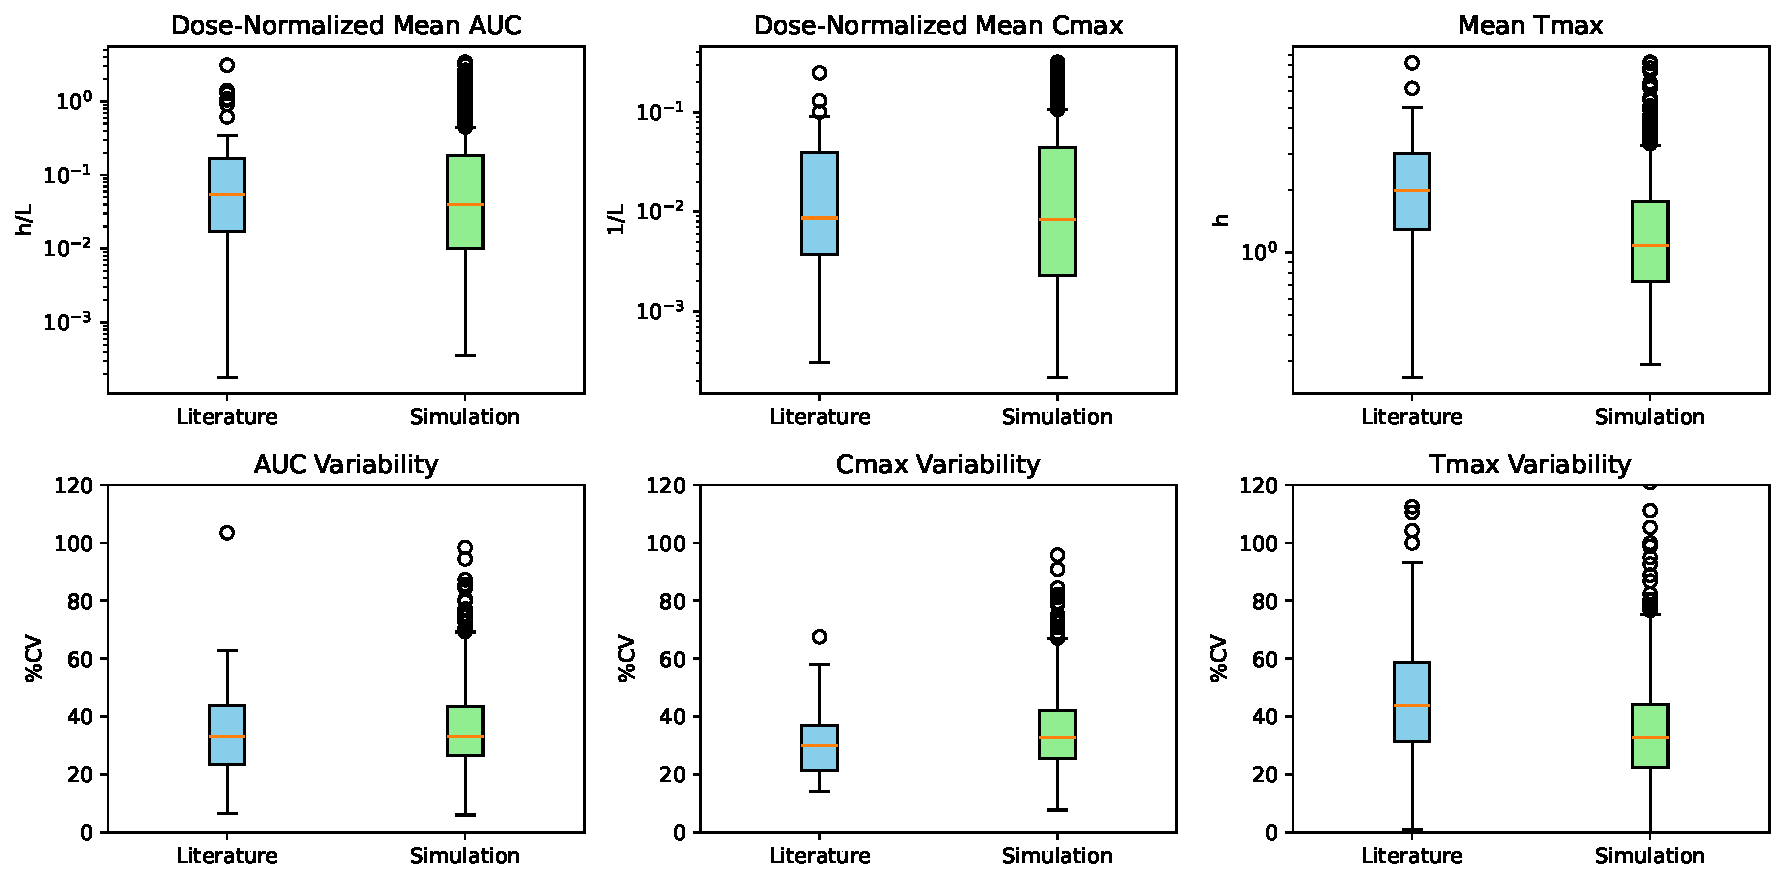
\includegraphics[width=\textwidth]{figures/pk-metrics-literature-vs-simulation.pdf}
    \caption{Comparison of three key PK characteristics (Mean/\%CV) between literature and 1000 simulated datasets.}
    \label{fig:benchmark}
\end{figure}

